\subsection{Kalibrierung des B-Feldes}
Es werden die vermessene Feldstärken und die zugehörigen Stromstärken aus Tabelle \ref{tab:eichung} mittels einer linearen Ausgleichsrechnung
\begin{equation}
  B(I) = B_0 + AI
\end{equation}
gefittet. Es ergibt sich der Graph aus Abbildung \ref{fig:eichung} und die Parameter
\begin{align}
  A &= (172,84 \pm 2,58)\si{\milli\tesla\per\ampere}\nonumber\\
  B_0 &= (-46,89 \pm 10,11)\si{\milli\tesla}
\end{align}

\begin{figure}
  \centering
  \includegraphics{build/feldeichung.pdf}
  \caption{Die gemessene Feldstärke in Abhängigkeit des angelegten Stroms}
  \label{fig:eichung}
\end{figure}
\subsection{Theoretische Lande-Faktoren der vermessenen Linien}
Für die rote Linie ist der Übergang $^1D_2\rightarrow ^1P_1$ verantwortlich.
Hierbei ist der Spin Null, daher ergibt sich nur der normale Zeeman mit $g_j=1$.
Für die blaue Linie ist der Übergang $^3P_1\rightarrow ^3S_1$ verantwortlich.
Hierbei ist der Spin Eins und es ergeben sich die $g_j$
\begin{align}
  0,5&(\pi)\nonumber\\
  1,5&(\sigma)\nonumber\\
  2&(\sigma)
\end{align}
Es ist zu erwarten, dass die beiden Lande-Faktoren für die $\sigma$-Ausrichtung sich zu $1,75$ überlagern werden.

\subsection{Dispersionsgebiet der Lummer-Gehrcke-Platte}
Mit den gegebenen Brechungsindizes
\begin{align}
  n(480\si{\nano\meter})&=1,4635\nonumber\\
  n(643,8\si{\nano\meter})&=1,4567
\end{align}
und der Formel \eqref{eqn:delta_lambda} lassen sich die Dispersionsgebiete
\begin{align}
  \Delta \lambda_{D,blau} &= 26,952\si{\pico\meter}\nonumber\\
  \Delta \lambda_{D,rot}  &= 48,913\si{\pico\meter}
  \label{eqn:dispersion}
\end{align}
berechnen

\subsection{Die rote Linie}
\begin{figure}
  \centering
  \begin{subfigure}{0.4\textwidth}
    \centering
    
\includegraphics[width=\textwidth]{Bilder/rot_sigma_ohne_B.JPG}
    \subcaption{Nicht aufgespalten}
  \end{subfigure}
  \begin{subfigure}{0.4\textwidth}
    \centering
    
\includegraphics[width=\textwidth]{Bilder/rot_sigma_mit_B.JPG}
    \subcaption{Aufgespalten $B=(0,644\pm 0,014)$T}
  \end{subfigure}
  \caption{Bilder der roten Linie}
  \label{fig:rote_Linie}
\end{figure}
Aus der Abbildung \ref{fig:rote_Linie} lassen sich die Werte in Tabelle \ref{tab:rote_Linie} ablesen.
Hier lässt sich mit den Gleichungen \eqref{eqn:delta_E}, \eqref{eqn:del_lambda} und \eqref{eqn:E_auf} lässt sich der Lande-Faktor
\begin{equation}
  g_j = 0,970\pm 0,022
\end{equation}
bestimmen.

\subsection{Die blau Linie}
\begin{figure}
  \centering
  \begin{subfigure}{0.4\textwidth}
    \centering
    
\includegraphics[width=\textwidth]{Bilder/blau_sigma_ohne_B.JPG}
    \subcaption{Nicht aufgespalten}
  \end{subfigure}
  \begin{subfigure}{0.4\textwidth}
    \centering
    
\includegraphics[width=\textwidth]{Bilder/blau_sigma_mit_B.JPG}
    \subcaption{Aufgespalten $B=(0,333\pm 0,012)$T}
  \end{subfigure}
  \caption{Bilder der blauen $\sigma$-Linie}
  \label{fig:blau_sigma_Linie}
\end{figure}

\begin{figure}
  \centering
  \begin{subfigure}{0.4\textwidth}
    \centering
    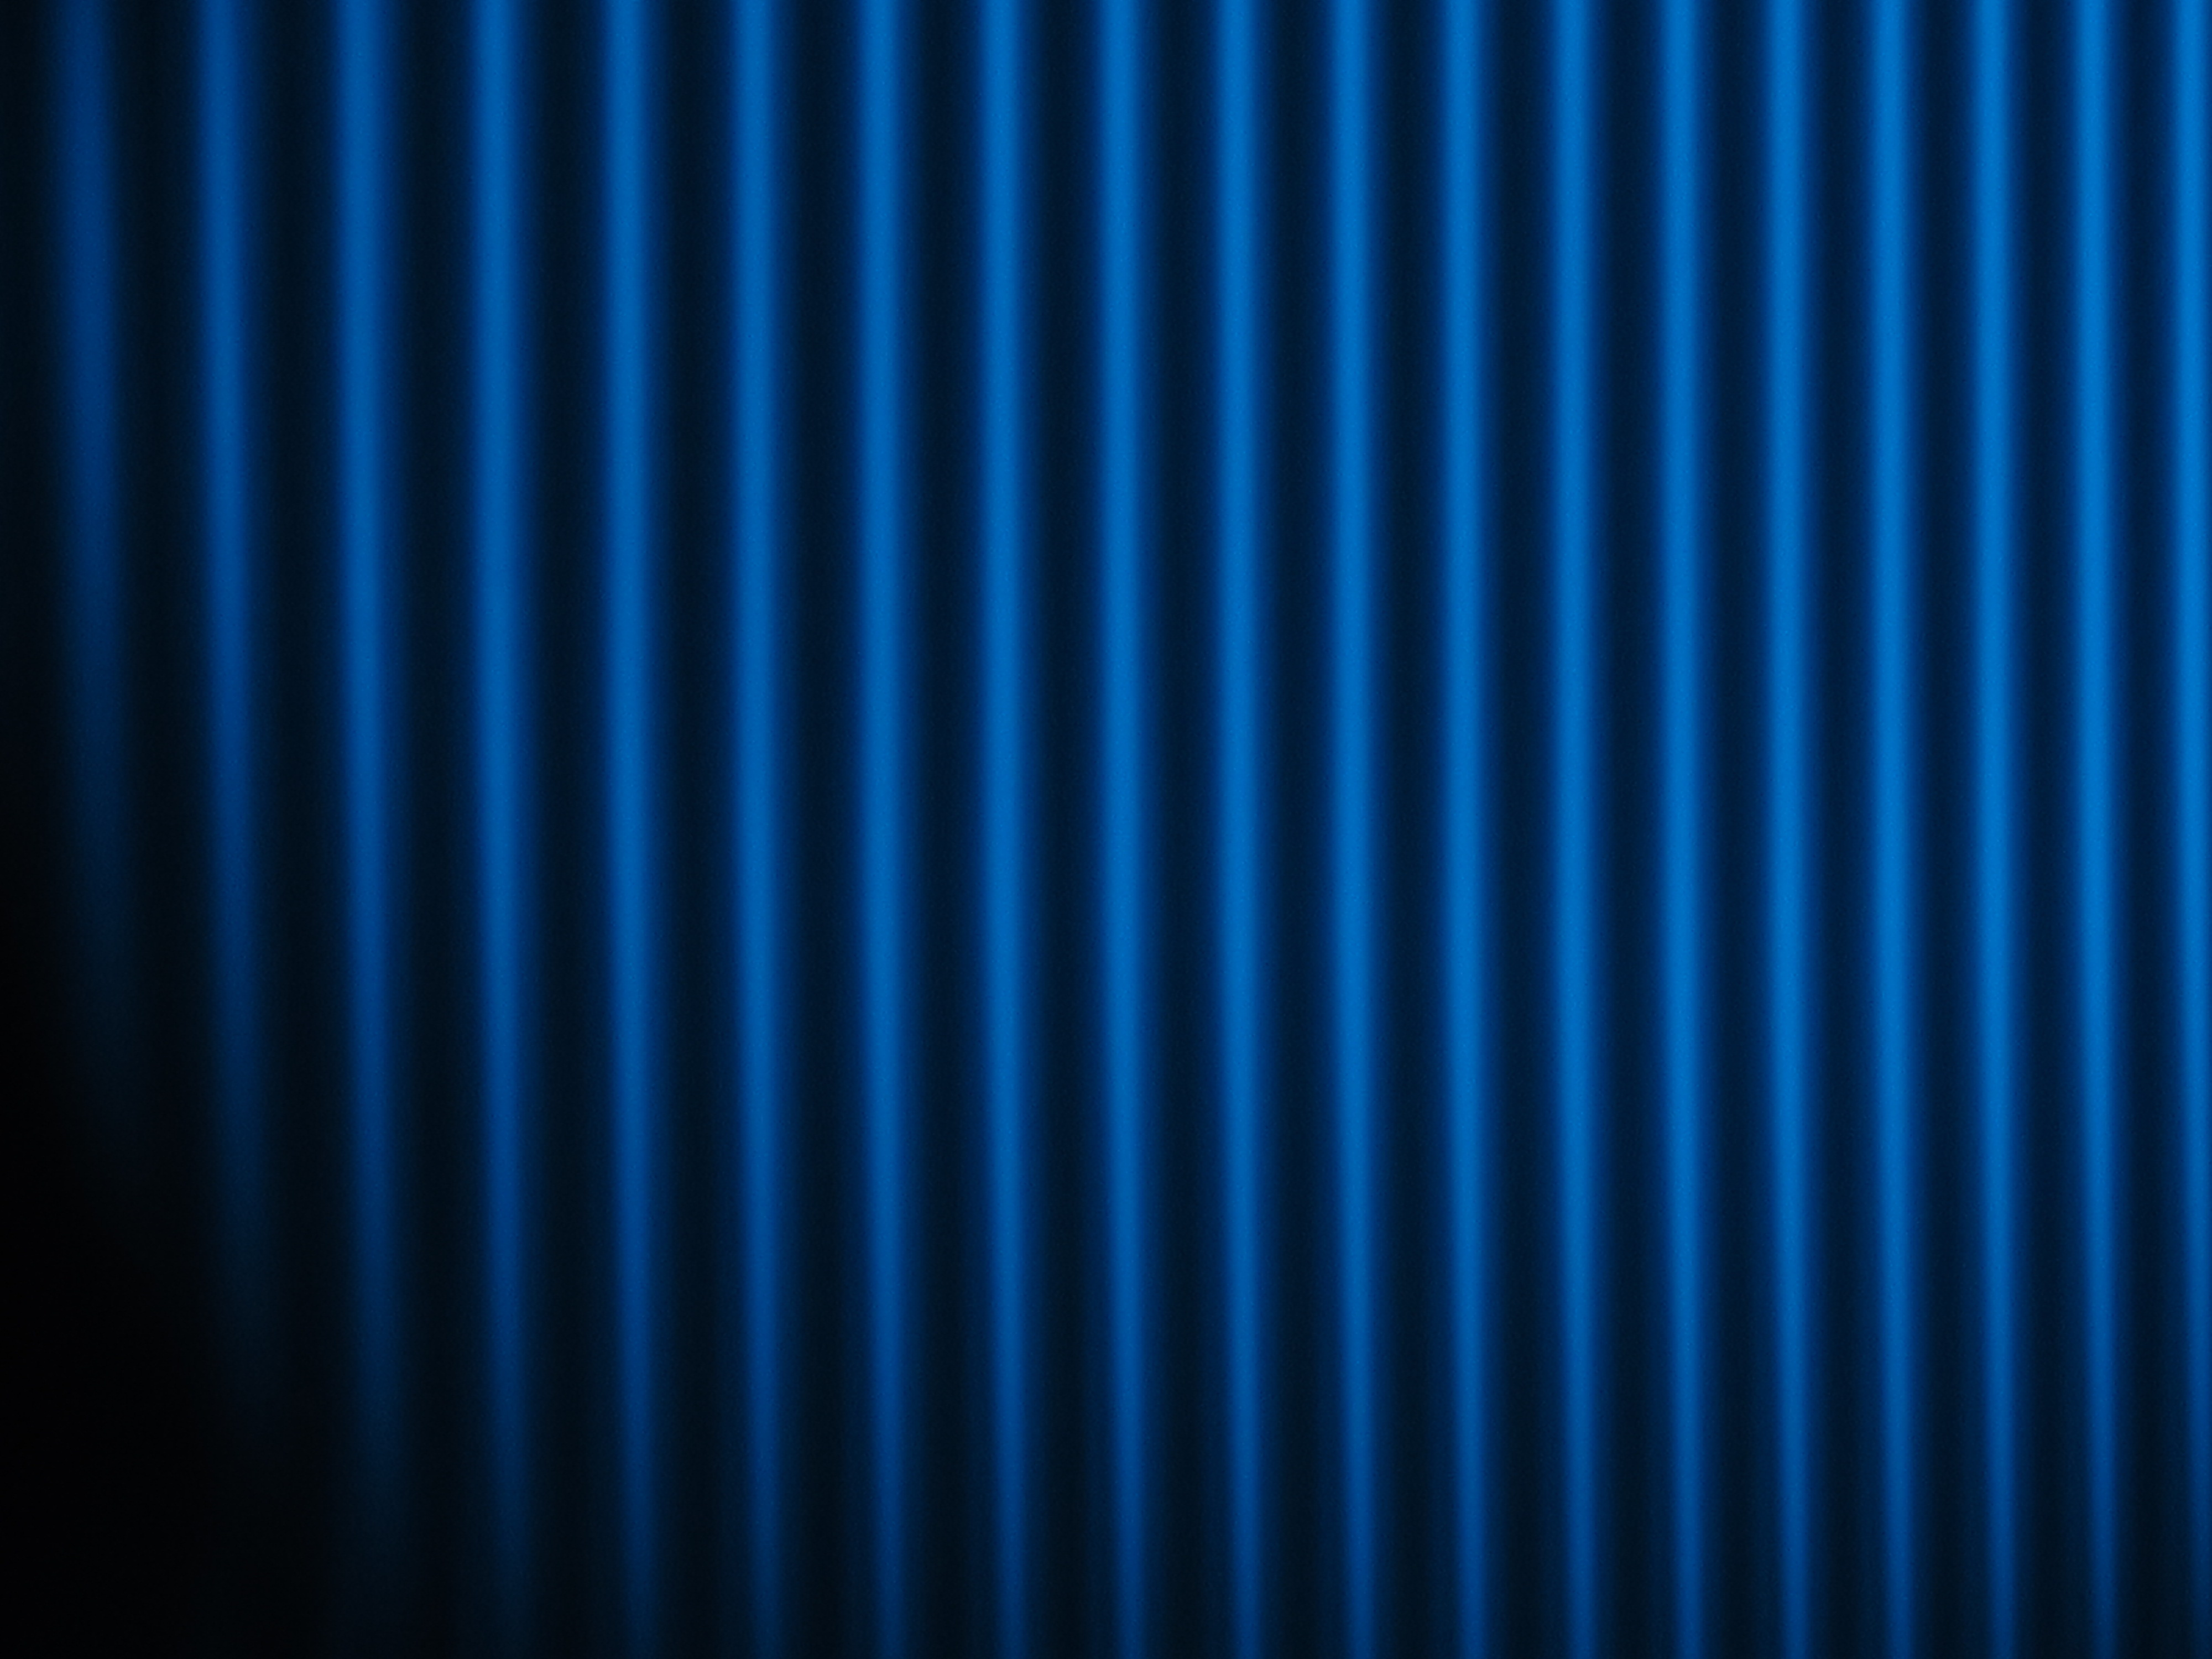
\includegraphics[width=\textwidth]{Bilder/blau_pi_ohne_B.JPG}
    \subcaption{Nicht aufgespalten}
  \end{subfigure}
  \begin{subfigure}{0.4\textwidth}
    \centering
    
\includegraphics[width=\textwidth]{Bilder/blau_pi_mit_B.JPG}
    \subcaption{Aufgespalten $B=(0,990\pm 0,018)$T}
  \end{subfigure}
  \caption{Bilder der blauen $\pi$-Linie}
  \label{fig:blau_pi_Linie}
\end{figure}
Analog zur roten Linie lassen sich aus den Abbildungen \ref{fig:blau_sigma_Linie} und \ref{fig:blau_pi_Linie} die Daten in den Tabellen \ref{tab:blau_sigma_Linie} und \ref{tba:blau_pi_Linie} ablesen
und die Lande-Faktoren
\begin{align}
  g_{j, \sigma} &= 1,78\pm 0,06\nonumber\\
  g_{j, \pi}    &= 0,548\pm 0,010
\end{align}
bestimmen.